\documentclass[10pt,a4paper,noendnumber=true]{scrartcl}
%german umlauts and localization
\usepackage[utf8]{inputenc} 
\usepackage[T1]{fontenc}
\usepackage[ngerman]{babel}
\usepackage[dvipsnames]{xcolor}
\usepackage{booktabs}
\usepackage{tabularx}

\usepackage{geometry}
\geometry{
	a4paper,
	total={170mm,257mm},
	left=20mm,
	top=20mm,
}

%figures etc.
\usepackage{graphicx}
\usepackage{standalone} %externalize files for faster compilation
\usepackage{float}

%mathematical symbols
\usepackage{latexsym} % special symbols 
\usepackage{amsmath,amssymb,amsthm}
\usepackage{textcomp} % supports the Text Companion fonts, which provide many text symbols (such as baht, bullet, copyright, musicalnote, onequarter, section, and yen)
%fonts:
%\usepackage{txfonts}  %supplies virtual text roman fonts using Adobe Times % needs to be loaded AFTER amsmath (because otherwise \iint is defined twice)
\usepackage{mathrsfs}  % for script-like fonts in math mode
\usepackage{nicefrac} % nice fracs in text
\usepackage{trfsigns}


%tables
\usepackage{tabularx}

%units
\usepackage{siunitx}
\sisetup{range-phrase=...}

% gescheiter Abstand nach paragraph
\newcommand{\properparagraph}[1]{\paragraph{\textcolor{Emerald}{#1}}\mbox{}\\}
\usepackage[parfill]{parskip}

% für die Auflistung von Vor- und Nachteilen in itemize-Umgebung
\newcommand\pro{\item[$+$]}
\newcommand\con{\item[$-$]}

%nice row vector
\newcommand{\rvect}[1]{\begin{bmatrix} #1 \end{bmatrix}}

\usepackage{subfig}

\title{Signalbehandling i ultralyd-avbildning}
\subtitle{Summary}
\author{Marvin Noll}
\date{2020 VÅR}

\begin{document}
\maketitle

\section{Lecture 1: Overview}

\subsection{Exam-Checklist}
\begin{itemize}
\item \textbf{Be able to use and understand the concepts power, amplitude, RMS, SNR, analog signal, digital signal.}

\begin{itemize}
\item Power: $P\propto A^2$
\item Amplitude $A$
\item RMS: root mean square $X_{RMS}=\sqrt{\frac{1}{T} \int\limits_{t_0}^{t_0+T} x^2(t)\; \text{d}t}$
\item Analog signal: $x(t) : \mathbb{R} \rightarrow \mathbb{R} $
\item Digital signal: sampled (and quantized) version of $x(t)$ : $x[n] : \mathbb{Z} \rightarrow \mathbb{Z},\mathbb{Q},...$
\end{itemize}

\item \textbf{Define the convolution operator and know the properties of convolution in Fourier space.}

The convolution of two functions is defined as
\begin{equation}
(f \ast g)(t) = \int\limits_{-\infty}^{+\infty} f(\tau)\,g(t-\tau)\;\text{d}\tau.
\end{equation}
\begin{equation}
(f \ast g)(t) \quad\laplace\quad F(f) \cdot G(f)
\end{equation}

\item \textbf{Explain what a filter is, and how a filter is applied as a convolution in time domain and a multiplication in the Fourier domain.}

A (passive) filter (with impulse response $g(t) \quad\laplace\quad G(f)$) attenuates parts of a signals spectrum $X(f)$:
\begin{equation}
y(t) = x(t) \ast g(t) \quad\laplace\quad Y(f) = X(f) \cdot G(f)
\end{equation}

\item \textbf{Be able to use and understand the filter properties stopband, passband, transition band, bandwidth, filter order. Also, explain the tradeoff between these properties.}

To achieve sharp transitions between stop and passband, high filter orders are needed. 

With the increasing of the length of the filter window, the spectrum becomes narrower, the ripples bunch more closely around the cut off frequency (but do not reduce the ripple magnitudes), the transition from passband to stopband becomes sharper. To reduce the ripples of the sidelobes, a proper filter should be used (like hamming window).

\item \textbf{Explain the difference between FIR filters and IIR filters.}

IIR filters use recursion and can become unstable but to achieve a given filter characteristic an IIR architecture usually requires a lower order than an FIR filter. FIR filter are always stable (Their impulse response is finite).

 \begin{figure}[H]
    \centering
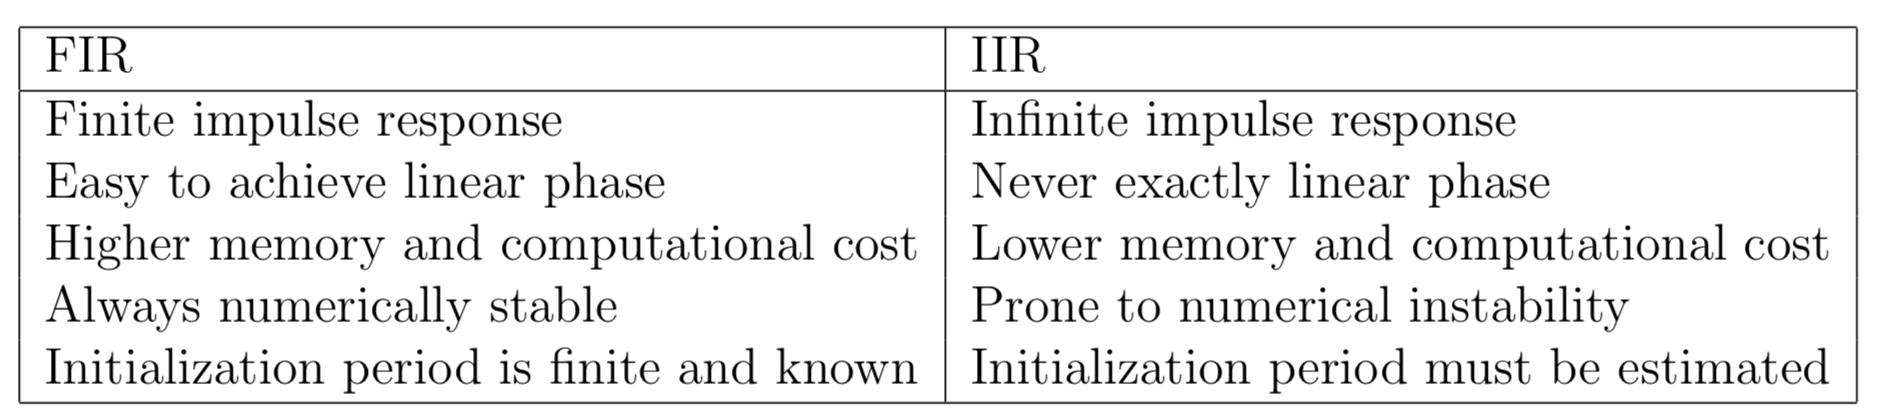
\includegraphics[width=0.7\textwidth]{img/FIR_IIR.png}
\renewcommand{\thefootnote}{\fnsymbol{footnote}}
\caption{FIR vs IIR} %\footnote[1]{Exercise 1 - Signal processing intro solution, Jørgen}} 
\end{figure}

\item \textbf{Explain what it means that a filter is linear, causal and shift invariant.}

\begin{itemize}
\item linear: scaled and sum inputs to the filter produces scaled and sum outputs with the same scaling factors.
\item causal: The filter does not use future values.
\item shift invariant: The properties of the filter do not change with absolute time.
\end{itemize}

\item \textbf{Be able to design filters for suppression of thermal noise based on the center frequency and signal bandwidth.}
\end{itemize}

\newpage
\section{Lecture 2: Intro Imaging}

\subsection{Exam-Checklist}
\begin{itemize}
\item \textbf{Explain the difference between transverse and longitudinal waves.}

\begin{itemize}
\item transverse: oscillates perpendicular to the moving direction (e.g. EM waves)
\item longitudinal: oscillates in the direction of travel (e.g. US sound waves)
\end{itemize}

\item \textbf{Understand the concept of logarithmic compression, and know in which settings logarithmic compression is useful.}
Logarithmic compression is used to enhance contrast and to show both weak and strong echos in the same image.

\item \textbf{Explain the concepts wavelength, frequency and speed of sound, and state the relation between these.}

The frequency of a wave $f$ (in \si{\hertz}) (or period $T$ (in \si{\s})) and its wavelength $\lambda$ (in \si{\m}) are related through the speed of sound $c$ (in \si{\m\per\s}) through

\begin{equation}
c =  \lambda \cdot f = \frac{\lambda}{T}.
\end{equation}

\item \textbf{State the relation between material properties compressibility, density and speed of sound. Know the typical speed of sound for soft tissue in the body.}

The speed of sound in a medium $c$ can be calculated by knowing the density of the medium $\rho$ (in \si{\kg\per\m\cubed}) and the compressibility $\kappa$ (in \si{\s\squared\m\per\kg}):
\begin{equation}
c=\frac{1}{\sqrt{\kappa\cdot\rho}}
\end{equation}

A typical value in soft tissue is $c=\SI{1540}{\m\per\s}$.

\item \textbf{Explaining the relation between acoustic impedance, reflection coefficient and transmission coefficient, stating the equations. Explain the usefulness of gel in ultrasound.}

The differences in acoustic impedances ($Z_{1,2}=\rho \cdot c$ (in \si{\kg\per\m\squared\per\s})) between two media 1 and 2 determine how much energy is transmitted/reflected.

The relative reflected energy is given by
\begin{equation}
\alpha_R = \left(\frac{Z_2-Z_1}{Z_2+Z_1}\right)^2.
\end{equation}
The transmitted portion is then $\alpha_T=1-\alpha_R$.

\textbf{The transducer is matched to tissue, but air has a tendency to get in the way. }

Gel is used to bridge the air gap between the transducer and the human skin (Impedance matching) to ensurre effective transmission of ultrasound. 

\item \textbf{Be able to explain the difference between scattering and specular reflection.}

\begin{itemize}
\item Specular: Reflections at large, smooth interfaces (between organs), amplitude not dependent on $f$
\item Scattering: Diverge/spreading of the beam with distance. Occurs for  Interfaces(within organs/tissue) smaller than $\lambda$, amplitude dependent on $f$
\end{itemize}

\item \textbf{Know which mechanisms lead to attenuation of ultrasound signal, and be able to estimate attenuation as a function of depth given the center frequency and the material properties of the medium.}

US waves are attenuated by \textit{absorption} and \textit{scattering}.

Attenuation is measured in \si{\dB\per\centi\meter\per\MHz}.

\item \textbf{Explain how a conventional B-mode image is constructed from several transmissions.}

The 2D sector is covered by steering the beam (phased array transducer) or scanning in 1D (linear array transducer).

\item \textbf{Explain the acquisition parameters center frequency, pulse length, aperture, focus, and image properties gain, resolution and SNR. Know the relations between acquisition parameters and image properties.}

\begin{itemize}
\item center frequency:"The center frequency of the resonant pass-band. Same as resonance frequency."
\item pulse length: "The length of the transmitted ultrasound pulse."
\item aperture: "The crossectional dimension of a wave source"/ the probe diameter
\item focus: "The region between the extreme nearfield and the farfield is called the transition.region. In this region the beam contracts before it starts to expand in the farfield, causing an apparent focusing that is referred to as diffraction focusing (The signal components from a certain depth are added in phase). The focusing is used to increase the signal intensity at a given depth and to improve the image lateral resolution."
\item gain: "
It is used an amplifier where the gain is swept as a function of time from low gain right after the pulse transmission when strong signals from shallow depths are received, towards higher gain when weaker signals from deeper.depths are received. This variation in gain compensates for the attenuation of the ultrasound in the tissue. "
\item resolution: 
\textbf{The apparent size in image is determined by the beam width and pulse length.}

1. radial/axial resolution: tells us how well the system can differentiate two targets placed at almost the same depth.

\textbf{2 scatterers at different depth will appear separate if separated by more than the pulse length.}

Ideally, the pulse length in imaging (B and M mode) should be as short as possible, but this is dependent on the physical properties of the probe. The pulse length is proportional to the spread of the frequencies(BW of the pulse): pulse length is proportional with 1/BW.

For imaging, the ideal pulse would be highest possible frequency (depending on the required depth penetration) and the shortest possible pulse length. 

2. lateral resolution: tells us how well the system can differentiate two targets placed at the same depth separated laterally. The lateral resolution of a beam is dependent on the focal depth, the wavelength and the probe diameter(aperture) of the ultrasound probe. 

The larger the aperture => the higher resolution of a line. 

The shorter the wavelength (the higher the frequency), the better the resolution, but there is a limitation given by the required depth penetration.

\textbf{2 scatterers at the same depth separated laterally by less than the beam width will appear as one.}

\textbf{If separated both laterally and in depth, they will appear as being in the same line, if lateral separation is within the beam.}

3. elevation resolution (normal to imaging plane-2D)

4. temporal resolution (frame rate) 
To imagine moving objects, structures such as blood and heart, the frame rate is important, related to the motion speed of the object. The eye generally can only see 25 FPS (video frame rate), giving a temporal resolution of about 40 ms. However, a higher frame rate and new equipment offers the possibility of replay at lower rate, f.i. 50 FPS played at 25 FPS, which will in fact double the effective resolution of the eye. 

In quantitative measurement, whether based on the Doppler effect or 2D B-mode data, sufficient frame rate is important to avoid undersampling.  In Doppler, the frame rate is also important in the  Nykvist phenomenon. 

The temporal resolution  is limited by the sweep speed of the beam. And the sweep speed is limited by the speed of sound, as the echo from the deepest part of the image has to return before the next pulse is sent out ad a different angle in the neighboring beam. "

\item SNR: "The ratio of the signal from the blood compared to the Gaussian noise from Brownian motion in the tissue, the transducer and the preamplifier."
\end{itemize}

\item \textbf{Understand and use the concepts frame rate, pulse repetition frequency, image region size, line density. Be able to calculate frame rate from the other parameters.}

\begin{itemize}
\item Frame rate: "The number of images per unit time. Typically more than 30 frames/sec for tissue imaging depending on the depth, while flow imaging can have frame rates below 10 frames/sec.

Tissue/flow image frame rate: To estimate the blood velocity we need several pulses in each beam direction; for tissue imaging a single pulse in each beam direction is sufficient. Because of this, the flow image frame rate is lower than the tissue image frame rate."
\item Pulse repetition frequency: "The repetition frequency of the transmitted pulses. This is the same as the sampling frequency."
\item Image region size:
\item line density:" The width of the echo will be determined by the beam width, and thus the distance between the beams (most ultrasound scanners today will intrapolate between beams if the distance between the beams is greater than the beam width). Ideally, the distance between the beam width should be the same as the beam width at the focal depth, for maximal resolution, thus lateral resolution of a beam determining \textbf{the line density}. This means that the line density would be suited to the beam width. This, however, holds only for a linear array."
\end{itemize}

\begin{equation}
framerate=
\end{equation}

\end{itemize}

\newpage
\section{Lecture 3: Pulse Echo Imaging}

\subsection{Exam-Checklist}
\begin{itemize}
\item \textbf{Understand the model describing the received signal as a convolution between the electrical impulse response, the transducer impulse response (twice) and a function describing the change of acoustic impedance in the medium.}

\begin{figure}[H]
\centering
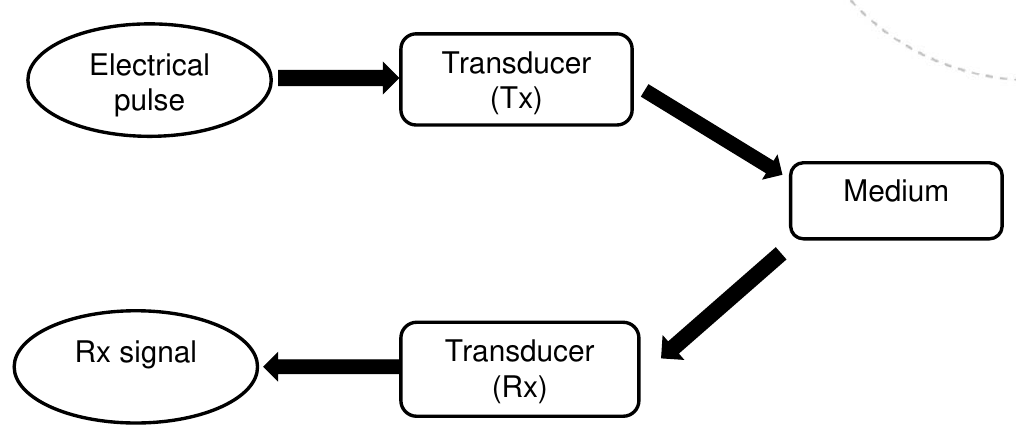
\includegraphics[width=0.5\textwidth]{img/pulseecho1.png}
\end{figure}

\item \textbf{Understand how the selection of center should match the transducer impulse response to achieve the best SNR.}

The transducer transfer function has a distinct maximum at its center frequency. That means any signal with a frequency away from the center frequency will be attenuated, thus reducing SNR.

\item \textbf{Understand how random positioning of scatterering objects leads to interference patterns consisting of destructive and constructive interference.}
"When two or more waves from different sources propagate through the same medium, they interfere with each other. That is, the effects of each individual wave are added at each point in the medium. The pressure at a point in the medium will be the sum of the pressures on it from the different waves. The constructive interference is referred to the case when the waves are in phase, as the amplitude is grater than that of both the individual waves. If the waves are in anti-phase, the effects of the waves can be canceled out (destructive interference). 

When a source generates a sound wave, the way in which the wave spreads out as it moves away from the source is determined by the relationship between the width and the source (the aperture) and the wavelength of the wave. If the aperture is smaller than the wavelength, the wave spreads out as it travels(diverges), an effect known as diffraction. For a sound wave from a small point source inside a medium, the wave spreads out as an expanding sphere (a spherical wave). The small scattering targets within tissue act as sources of such spherical waves. 

If the width of the source is much greater than the wavelength of the wave, the waves are relatively flat(plane) rather tan curved and lie parallel to the surface of the source. Such waves travel in a direction perpendicular to the surface of the source with relatively little sideways spread, in the form of a parallel-sided beam. 

These 2 different cases of curved waves from a small source and plane waves can be linked by considering the large source to be made up of a long row of small sources. Each of the small sources generates a sound wave of the same frequency and amplitude and all are in phase with each other. The curved waves from each propagate outwards and the parts of the curve which are parallel to the surface of the source align to from plane waves. The other, non-parallel parts of the curved waves tend to interfere destructively and cancel out. "

\item \textbf{Understand the concept of correlation length and its relation to pulse length and resolution.}
\end{itemize}

\newpage
\section{Lecture 4: Acoustic Field}

\subsection{Exam-Checklist}
\begin{itemize}
\item \textbf{Explain what a piezoelectric material is, and know the function of the matching layer and the backing layer.}
\begin{itemize}
\item Piezoelectric material converts electricity into mechanical displacement
\item Matching layer: $\lambda/4$ thick material with mechanical properties between the piezo and tissue. Increases coupling; ringing dies down more quickly
\item Backing layer: Heavy block of material. Dampens down ringing
\end{itemize}


\item \textbf{Know that transducer elements become directional for small wavelengths.}
\begin{itemize}
\item $d \ll \lambda$: Emitting uniformly in all directions
\item $d \approx \lambda$ : Emitting more to the front
\end{itemize}

\item \textbf{Explain the difference between Continuous wave (CW) and Pulsed Wave (PW) imaging.}
\begin{itemize}
\item CW: expected diffraction/interference profile
\item PW: interference at different spatial locations (for different frequencies) $\rightarrow$ smoothes out beam profile
\end{itemize}


\item \textbf{Explain how, by using Huygens principle, the transducer surface may be modeled as a collection of point sources, and how this leads to the Rayleigh-Sommerfeld integral.}
\begin{itemize}
\item Huygens principle: wave front is sum of many point sources
\item Rayleigh-Sommerfeld integral sums these point sources weighted with the velocity at the transducers surface
\end{itemize}


\item \textbf{Explain what the Fresnel approximation is (what is the underlying approximation).}

The Fresnel approximation of the Rayleigh-Sommerfeld integral uses a binomial approximation for the distance to the transducer


\item \textbf{Know how the Fraunhofer approximation relates the transducer aperture function and the ultrasound field in a plane parallel to the transducer. Also, know when the approximation is valid, considering both the unfocused and focused case.}
\begin{itemize}
\item The Fraunhofer approximation shows, the diffraction pattern in the far field to be proportional to the Fourier transform of the transducer aperture velocity distribution
\item The approximation is valid in the far field or in the focus of a focused beam
\end{itemize}

\item \textbf{Explain why we get some focusing at some depth, even when not focusing the beam.}

Due to diffraction, the beam will converge first and than expand in the far field. The converging is called diffraction focusing.

\item \textbf{Explain what the F-number is, and be able to use the F-number to quantify the spatial extent of the transmitted ultrasound field in lateral and elevation directions. Also, know about the tradeoff between resolution and depth of focus.}
\begin{itemize}
\item $F\#=\frac{\text{focal depth}}{aperture width}=\frac{F}{D}$
\item $F\#$ small: narrow beam, high lateral resolution, low depth of focus
\item $F\#$ large: wide beam, low lateral resolution, high depth of focus
\end{itemize}

\item \textbf{Explain what apodization is, and how it effects the main lobes and side lobes in the field.}

Apodization means weighting of the transducer elements amplitude. As weighting functions, windows, like Hann/Hamming are used. No apodization means using a rectangular window.

Apodization is used to suppress side lobes, but widens the main lobe as a side effect.
\end{itemize}

\subsection{Formula}
\subsubsection{Unfocused beam}
Crossover from near field to far field (Transducer width $D$, wavelength $\lambda$):
\begin{equation}
R_c = \frac{D^2}{\lambda}
\end{equation}

Beamwidth a depth $z$:
\begin{equation}
\frac{z}{D}\cdot\lambda
\end{equation}

\subsubsection{Focused beam}
F-number (Transducer width $D$, distance to focus $F$):
\begin{equation}
F\# = \frac{F}{D}
\end{equation}

Beam width in focus:
\begin{equation}
D_F=1.2 \cdot F\# \cdot \lambda
\end{equation}

Depth of focus (i.e. focal length):
\begin{equation}
L_F = 2 \cdot F\#^2 \cdot \lambda
\end{equation}

\newpage
\section{Lecture 5: Signal Processing Chain}

\subsection{Exam-Checklist}
\begin{itemize}
\item \textbf{Be able to list and briefly explain the function of the following elements in the signal processing chain: Transmit pulse generator, T/R-switch, transducer, Time Gain Compensation (TGC), Analog-to-digital converter (ADC), beamforming, demodulation, envelope detection, scan conversion, and compression.}
\begin{itemize}
\item Transmit pulse generator: generates a (ideal) electrical pulse sequence
\item T/R-switch: switches the transducer between transmitting and receiving; protects amplifier from send pulses
\item transducer: uses piezo-electric material to convert electrical signals in vibrations and vise versa
\item TGC: amplifies later signal parts more thus compensates for greater attenuation in greater depths. Is used before ADC to limit needed quantization steps for the ADC (cheaper)
\item ADC: converts the analog receive signals into a digital waveform
\item beamforming: control interference pattern, to e.g. do dynamic focusing on receive
\item demodulation: removes carrier frequency, transforms signal to baseband (saves memory space)
\item envelope detection: remove oscillations from signal
\item converts beam space ($\# of beams \times depth$) to image space ($x \times depth$). Does perform 2D radial interpolation.
\item used to see stronger and weaker features in the same image
\end{itemize}

\item \textbf{Explain what demodulation is, and why it is useful. Know about two techniques for implementing demodulation.}

Demodulation means converting the received passband signal to its baseband representation. This two step process is either done by applying the Hilbert transform (removes negative frequencies) and downmixing (shifts the signal from $f=f_c$ to $f=0$) or by downmixing first and then passing the signal through a lowpass filter (to remove the spectrum around $f=-2\,f_c$)

\begin{figure}[H]
\centering
\subfloat[RF Spectrum]{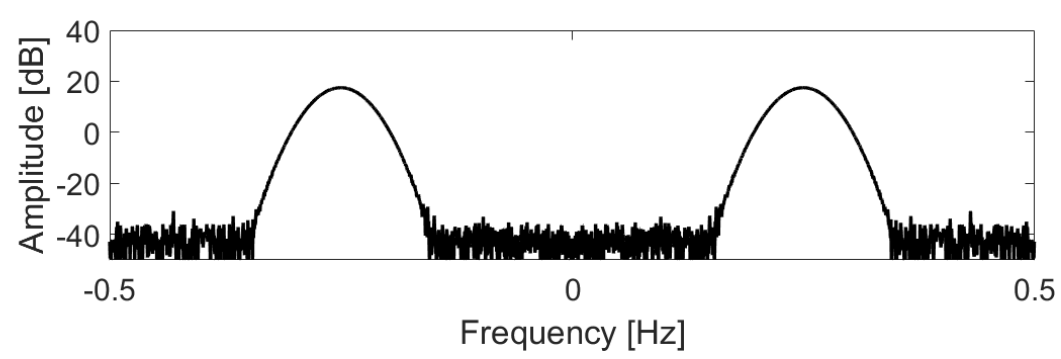
\includegraphics[width=0.45\textwidth]{img/demo1.png}}
\\
\subfloat[Hilbert]{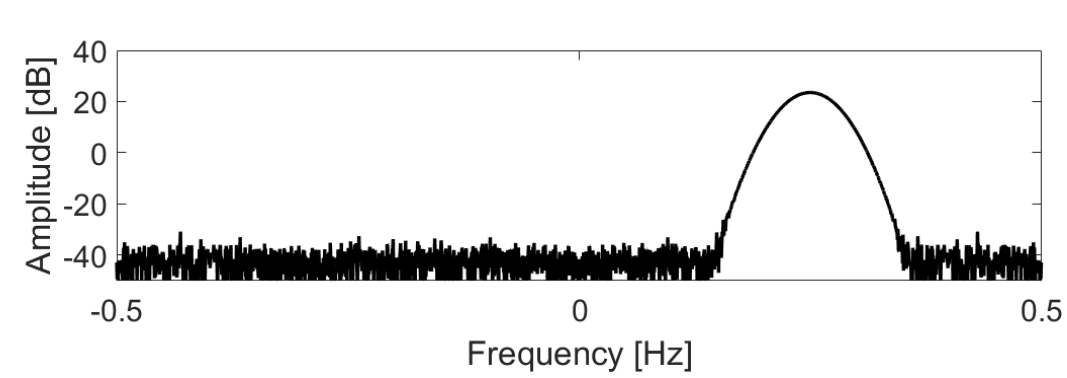
\includegraphics[width=0.45\textwidth]{img/demoh1.png}}
\qquad
\subfloat[Downmix]{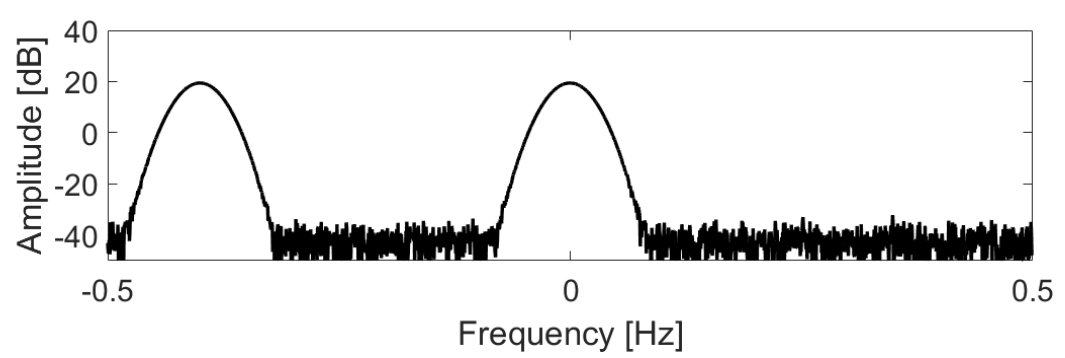
\includegraphics[width=0.45\textwidth]{img/demolp1.png}}
\\
\subfloat[Hilbert + Downmix]{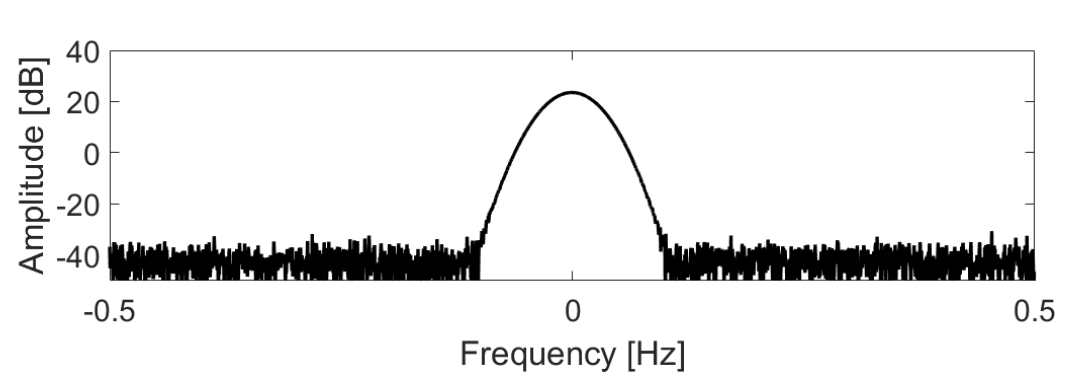
\includegraphics[width=0.45\textwidth]{img/demoh2.png}}
\qquad
\subfloat[Downmix + Lowpass]{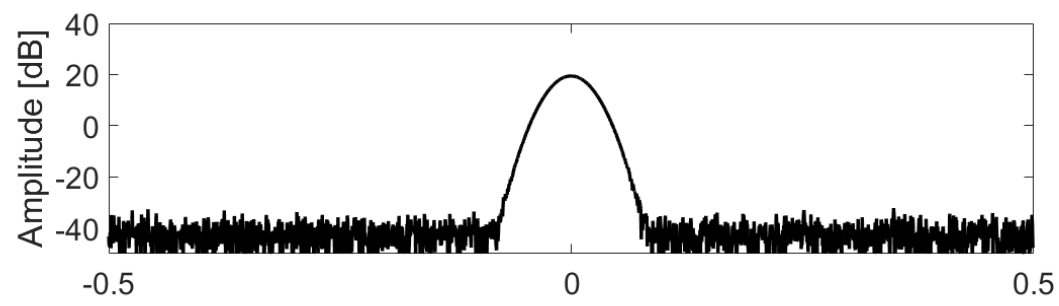
\includegraphics[width=0.45\textwidth]{img/demolp2.png}}
\end{figure}

\item \textbf{Understand and use correctly the terms RF signal, pre-envelope, IQ signal, envelope, beam space, gain and dynamic range.}
\begin{itemize}
\item RF-signal: (real) received passband signal with energy around $f=\pm f_c$
\item Pre-envelope: (complex) passband signal with energy only around $f=+ f_c$
\item IQ-signal: (complex) baseband signal with energy only around $f=0$
\item envelope: IQ-signal ``without oscillations" $A(t)=\left|s_{IQ}(t)\right|$
\item beam space: 2D signal (beam number $\times$ depth) after beam forming
\item gain/dynamic range: gain $\hat{=}$ brightness of the image; dynamic range influences contrast: higher: see weaker signals, but fewer nuances
\end{itemize}


\item \textbf{Explain what happens in the frequency domain when a time domain signal is multiplied by a 1) real-valued amplitude signal, 2) signal with constant amplitude, but linearly varying phase.}
\begin{enumerate}
\item $x(t) \cdot y(t) \quad\laplace\quad X(t) \ast Y(t)$
\item $x(t) \cdot \e^{-i 2 \pi f_0 t} \quad\laplace\quad X(f-f_0)$
\end{enumerate}


\item \textbf{Explain what Time-Of-Flight (TOF) is, and how it is used in Delay-And-Sum (DAS) beamforming. Be able to calculate the TOF from a given geometry.}

To sum the signals from all transducer element, a delay has to added to each signal compensation for the different path lengths between the element and the scatter source. The time it takes the sound to travel these paths is called time of flight (TOF).

It includes the time from the $tx$ transducer element to the point scatter and from there back to one of many transducer elements:
\begin{equation}
TOF = t_{tx} + t_{rx}
\end{equation}

The time to the point is (depth of point $z$, speed of sound $c$)
\begin{equation}
t_{tx} = \frac{z}{c}.
\end{equation}

The time back to an element (index $e$) is (coordinate of point $(x,z)$, location of transducer element $x_e$)
\begin{equation}
t_{rx} = \frac{\sqrt{(x-x_e)^2+z^2}}{c}.
\end{equation}

\begin{figure}[H]
\centering
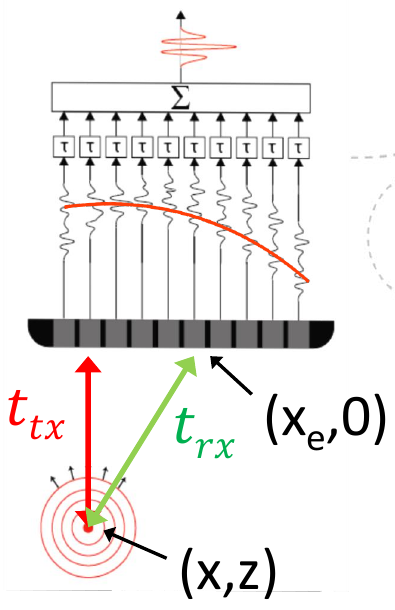
\includegraphics[width=0.25\textwidth]{img/tof.png}
\end{figure}
\end{itemize}

\newpage
\section{Lecture 6: Beamforming}

\subsection{Exam-Checklist}
\begin{itemize}
\item \textbf{Explain what grating lobes are, and how we may avoid or reduce them. Under what conditions can we guarantee no grating lobes?}

Grating lobes are lobes ever further out that side lobes. They are caused by interference between the pulses from neighboring transducer elements. They cause signal leakage.

Without steering they can be avoided, if the element pitch $d$ is smaller than the wavelength $\lambda$:
\begin{equation}
d<\lambda
\end{equation}

When steering is used, they can be avoided, if the pitch is smaller than half the wavelength:
\begin{equation}
d<\frac{\lambda}{2}
\end{equation}

\item \textbf{Explain what dynamic focusing is, and why this is easier to achieve on receive than on transmit.}

On transmit, the beam can be focused by adding delays to the elements in order to create a concave curved wavefront. To do this, the desired focal point has be be known in advance.

To do beamforming on receive, the delays can be added \textit{after} receiving the signal. Thus the focal point can be chosen freely (this is called TOF beamforming).


\item \textbf{Explain how delays may be adjusted to steer the beam, and why the use of steering may lead to more grating lobes, smaller effective aperture and reduced SNR.}
If the delay for each element from one side of the transducer to the other is increased continuously, the resulting beam is deflected to one side (as a result of the Huygens principle).

If steering is used, the steer angle introduces additional lag for some directions.

%TODO


\item \textbf{Explain how apodization affects the main lobe and sidelobes.}
Apodization is the method of applying a weightning window to the transducer elements.

Using another window (Hann/Hamming/Tukey/...) than the default rectangular apodization can be useful to supress side lobes but it comes with widening the main lobe.


\item \textbf{Calculate the lateral resolution in the image from center frequency, active aperture size on transmit and receive.}

Lateral resolution is approximately equal to the beam width (in focus) $D_F$:
\begin{align}
D_F &= 1.2 \, F\#_{txrx} \, \lambda \\
D_F &= 1.2 \left(\frac{1}{F\#_{tx}}+\frac{1}{F\#_{rx}}\right)^{-1} \, \lambda\\
D_F &= 1.2 \left(\frac{1}{F\#_{tx}}+\frac{1}{F\#_{rx}}\right)^{-1} \, \frac{c}{f}\\
\end{align}


\item \textbf{Explain what expanding aperture is, and why this is useful.}

Use a wider aperture for greater focal depth than for shallow ones to achieve uniform resolution over the whole depth range.

\end{itemize}

\newpage
\section{Lecture 7: Linear Imaging Systems}

\subsection{Exam-Checklist}
\begin{itemize}
\item \textbf{Explain what it means that an imaging system in linear shift invariant, and know that imaging in such a system may be described as a convolution between the object and a point spread function (PSF).}

Shift in-variance means, that the characteristics of the imaging system do not change depending on the object position $o(x,z)$. Because the imaging system is also assumed linear, it qualifies as an LSI (LTI) system and thus can be modeled with a point spread function. The image $i(x,z)$ is then
\begin{equation}
i(x,z) = o(x,z) \ast psf(x,z).
\end{equation}

\item \textbf{Understand how 2D imaging may be described as multiplication with the Fourier transform of the PSF in the spatial Fourier domain (k-space).}

\begin{equation}
I(f_x,f_z) = O(f_x,f_z) \cdot Psf(f_x,f_z)
\end{equation}

\item \textbf{Know that any 2D image may be represented as a sum of single frequency spatial images.}

Because the image and the spectrum form a (2D) Fourier pair.

\item \textbf{Be able to calculate the 2D Fourier transform of an image or spatial function and apply the correct axes in k-space.}

(Inverse relationship between $(x,z)$ and $(f_x,f_z)$)

\end{itemize}

\newpage
\section{Lecture 8: Image Formation}

\subsection{Exam-Checklist}
\begin{itemize}
\item \textbf{Be familiar with the different types of array geometries and their corresponding applications.}

\begin{itemize}
\item Linear array: high resolution/high freq., limited width 
	\\$\Rightarrow$ carotid arteries
\item Curved array: large image width, large near field
	\\$\Rightarrow$ Abdominal examinations
\item Phased array: small footprint, 90 deg sector format, lower freq.
	\\$\Rightarrow$ cardiac imaging
\end{itemize}

\item \textbf{Explain the differences and relations between the transmit spatial impulse response, the receive spatial impulse response and the pulse echo response.}

\begin{figure}[H]
\centering
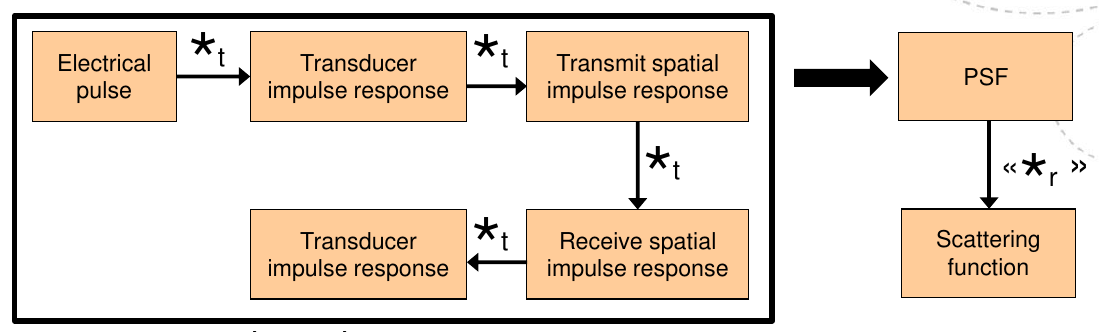
\includegraphics[width=0.8\textwidth]{img/psf.png}
\end{figure}

\item \textbf{Explain how the point spread function is found by sampling the pulse echo response at a specific time point and position. Which time point and position?}
\begin{equation}
PSF=h_{pe}(TOF,x_f-\vec{x})
\end{equation}


\item \textbf{Be able to describe the PSF quantitatively in $k$-space. More specifically, be able to calculate the center frequency and bandwidth in $k_x$ and $k_z$-dimensions.}



\item \textbf{Understand what speckle is, and how speckle size relates to the size of the PSF in space and k-space.}

Speckles are present in regions with non structured scatterers.


\end{itemize}

\newpage
\section{Lecture 9: Doppler I}

\subsection{Exam-Checklist}
\begin{itemize}
\item \textbf{Explain what Rayleigh scattering is, and know the relation between center frequency and backscattered signal amplitude from blood.}

Rayleigh scattering is scattering from small particles ($<\lambda$). The scattered waves have an amplitude $\propto f^4$.

\item \textbf{Explain how blood flow volume may be estimated using ultrasound, and how the pressure drop across a stenosis may be estimated from the measured velocity.}

The blood flow through a vessel with diameter $A_1$ (measured with ultrasound imaging) and velocity $v_1$ (measured with Doppler ultrasound) is
\begin{equation}
Q_1 = v_1 \cdot A_1
\end{equation}

The pressure drop over a stenosis can be expressed as
\begin{equation}
P_1 - P_2 \approx 4\,v_2^2
\end{equation}
if $v_2 \gg v_1$.

\item \textbf{Explain what the Doppler shift is, and be able to calculate the Doppler shift from the transmitted center frequency and blood velocity.}

The Doppler shift is a shift in observed frequency of a wave reflected from an object due to relative movement between the observer and the observed object.

The Doppler shift $f_d$ is (center frequency $f_0$, speed of sound $c$, velocity of the particle $\nu$ and observation angle $\theta$)
\begin{equation}
f_d = \frac{2\,\nu\,\cos\,\theta}{c}\,f_0
\end{equation}

\item \textbf{Explain what the Doppler power spectrum is. What is the interpretation of each value in the spectrum?}

The Doppler power spectrum is the result of a short time Fourier transform, i.e. it is a spectogram. It shows velocity over time with the intensities shown as color/grayscale pixels.

\item \textbf{Be able to calculate the Doppler power spectrum from the correlation function.}



\item \textbf{Know that the Doppler power spectrum is subject to variance, and know how to reduce this variance?}


\end{itemize}

\newpage
\section{Lecture 10: Doppler II}

\subsection{Exam-Checklist}
\begin{itemize}
\item \textbf{Understand and use correctly the terms fast-time and slow-time, aliasing, Nyquist velocity, and baseline shift.}
\begin{itemize}
\item Fast time: The RF signal sampled at $\approx \SI{50}{\MHz}$
\item Slow time: One sample of the fast time signals of one depths, sampled at $\approx \SIrange{0.1}{20}{\kHz}$
\item Aliasing: If the actual velocity exceeds the Nyquist velocity limit, frequency/velocity wrap around will occur. 
\item Nyquist velocity:
The Nyquist velocity is the fastest velocity that can be measured with PW Doppler without aliasing effects.

it can be calculated by (speed of sound $c$, the pulse repetition frequency $PRF$ and the center frequency $f_0$)
\begin{equation}
\nu_\text{Nyq} = \frac{c\,PRF}{4\,f_0}.
\end{equation}
\item Baseline shift: Zero frequency line of the spectrum is shifted manually
\end{itemize}



\item \textbf{Explain why the measured Doppler shift depends on the angle between the beam and the velocity of the scatterer.}

Doppler shift only occurs for waves moving to or from the observer. So the strongest shift is visible for an angle of $\theta=\SI{0}{\degree}$.

In detail, for doing Doppler measurements, only the projected velocity
\begin{equation}
\nu_d=\nu \, \cos \theta
\end{equation}
is regarded.

\item \textbf{Explain how the Nyquist velocity limits the range of measurable velocities, and how the measurable velocity range may be altered by stacking spectra and using baseline shift. Be able to calculate the Nyquist limit from the PRF and center frequency.}

The Nyquist velocity is the (absolute) maximum observable velocity without aliasing.

If aliasing occurs, stacking the spectra on top of each other can virtually augment the maximum/minimum velocity range and thus allow the operator to (visually) get a measurement after all.


\item \textbf{Explain the importance of window functions when performing spectral estimation.}

Window functions are used to suppress sidelobes (visually smoothing the spectrum).

\item \textbf{Explain why the PRF is limited by the image depth, and calculate the maximum possible PRF.}

Each measurement takes a least the TOF to the target and back to the transducer. This limits the maximum possible PRF to (speed of sound $c$, depth of target $z$)
\begin{equation}
PRF_{max} = \frac{c}{2\cdot z}
\end{equation}

\item \textbf{Know how velocity resolutions limited by temporal observation window, PRF and center frequency.}

The velocity resolution is (speed of sound $c$, the pulse repetition frequency $PRF$ and the center frequency $f_0$, size of window function in samples $N_\text{window}$)
\begin{equation}
\Delta\nu = \frac{2\cdot\nu_\text{Nyq}}{N_\text{window}} = \frac{2\,c\,PRF}{4\,f_0\,N_\text{window}}
\end{equation}

\item \textbf{Explain what spectral broadening is, why it occurs, and how this may also limit velocity resolution.}

Due to the inverse relationship between time and bandwidth, the spectrum becomes broader, if the observation time becomes smaller (due to beam-to-flow angle, pulse length, ...)

\item \textbf{Explain what clutter filtering is, and be able to implement clutter filtering of signals.}

The so called clutter signal results from the surrounding tissue. It has components around $f=0$ since it's mostly stationary or slowly moving.

To remove the clutter signal, a highpass filter on the slow time signal is used. This is especially needed for mean velocity estimators, because the clutter can shift the mean velocity towards zero.

\end{itemize}

\newpage
\section{Lecture 11: Color Flow}

\subsection{Exam-Checklist}
\begin{itemize}
\item \textbf{Explain what Color Flow Imaging (CFI) is, and how this modality is complementary to PW Doppler.}

In comparison to PW/CW, color flow is used to qualitatively show blood flow in a 2D sample volume. After getting an overview with color flow, PW Doppler can be used to get a quantitative measurement of a smaller sample volume.

\item \textbf{Explain and use correctly terms packet size, interleaving, firing rate, Doppler PRF, autocorrelation function, segmentation/arbitration.}
\begin{itemize}
\item Packet size: Number of firings in one direction per packet %TODO
\item Interleaving: Increasing framerate by interleaving packets %TODO
\item Firing rate: Time interval between firings
\item Doppler PRF: Time interval between firings in the same direction
\item Autocorrelation function: Measures similarity of a signal with itself as a function of time lag
\item Segmentation/Arbitration: Showing B-mode image or color flow pixels depending on e.g. blood/tissue/noise indicators
\end{itemize}

\item \textbf{Be able to define and use the autocorrelation estimator. Under which assumptions is the autocorrelation estimate unbiased?}

The autocorrelation of $s(t)$ is given as (lag $\tau$, expected value operator $\langle \cdot \rangle$)
\begin{equation}
R_s(\tau) = \langle s(t) \cdot s(t+\tau) \rangle
\end{equation}

Inside the Nyquist frequency interval, the autocorrelation is an unbiased estimator for the velocity.

\item \textbf{Be able to convert between phase shift and velocity of the scatterer, given the PRF and center frequency.}

Using the phase shift $\angle R(1)$, the velocity is (speed of sound $c$, pulse repetition frequency $PRF$, center frequency $f_0$)
\begin{equation}
\nu = \frac{\angle R(1)\,PRF\,c}{4\,\pi\,f_0}
\end{equation}

\item \textbf{Explain what duplex imaging is, and describe the acquisition scheme.}

Acquire B-mode and Doppler measurements in turns.

\item \textbf{Explain all steps in the CFI processing chain: Acquisition, processing, display. Describe the acquisition scheme (duplex with B-mode and CFI). Why do we use a packet-based acquisition? How do we process the acquired data to obtain mean velocity estimates in each image point?}



\item \textbf{Explain why clutter filtering is more important and more difficult in CFI than in PW Doppler.}

Color flow imaging (CFI) displays mean velocities. With the clutter signal, the mean velocity estimator is biased towards zero.

\item \textbf{Be able to calculate the frame rate and Doppler PRF given a description of the acquisition (firing rate, number of interleave groups, packet size, number of B-mode firings.}



\item \textbf{Explain what regression filters are. What is the motivation for using regression filters instead of FIR filters for small packet sizes?}



\item \textbf{How to select which image points should display B-mode or velocity estimates?}

\begin{itemize}
\item Show blood, if...
\begin{itemize}
\item High power Doppler signal (after clutter filter)
\item Low power in B-mode image
\end{itemize}
\item Show Tissue, if...
\begin{itemize}
\item Low power Doppler signal (after clutter filter) %TODO frequency/power?
\item High power in B-mode image
\end{itemize}
\end{itemize}

\item \textbf{Be aware of the following limitations of CFI: Flashing artifacts, color blooming, manual angle correction, aliasing, clutter filtering bias and high variance.}
\begin{itemize}
\item Flasing artifacts: False coloring of tissue due to insufficient filtering (slow blood or moving tissue/probe)
\item Color blooming: CFI color overlay leaks/blooms into surrounding tissue
\item Manual angle corrections: Needed, because only the axial velocity component is measured
\item Aliasing: Velocity exceeds Nyquist limit
\item Clutter filter bias: Bias due to clutter prevents qualitative measurements
\item High variance: prevents qualitative measurements
\end{itemize}


\item \textbf{Understand the tradeoff between spatial resolution and SNR, and the tradeoff between temporal resolution, lateral sampling density and estimator accuracy.}


\end{itemize}


\newpage
\section{Lecture 12: Alternative velocity estimators}

\subsection{Exam-Checklist}
\begin{itemize}
\item \textbf{Explain what it mean that the autocorrelation approach is a narrow-band technique.}

Autocorrelation uses only a small portion of the available signal information.

The variance of the velocity estimation is small for a small bandwidth $B$ (packet size $N$):
\begin{equation}
\text{var}(\bar{\omega}_d) = \frac{B}{N}
\end{equation}

\item \textbf{Explain briefly how mean velocity estimation is performed when using cross-correlation and speckle tracking.}

Cross correlation uses the fast time RF signals. From the $arg max$ of the cross correlation, the velocity can be calculated.

In speckle tracking, the displacement of the speckles originating from the blood are compared from one frame to the next. With the framerate, velocity can be calculated.

\item \textbf{Explain what tracking Doppler is. Which limitation of spectral velocity estimation is addressed by tracking Doppler?}

To decrease spectral broadening, longer temporal observation windows are needed.

If the beam-to-flow angle is known, the sample volume can track the blood movement across multiple frames.

\item \textbf{Explain what plane wave imaging is and how this technique can be used to increase the frame rate. Be aware of the limitations of plane wave imaging (resolution, axial lobes, motion artifacts).}

Instead of sending/receiving consecutive beams to scan the field of view, all elements send at once. By using delays, multiple angled planar waves are used instead of the narrow beams.

After dynamic focusing and parallel beamforming on receive, there are many low resolution images. They can be summed coherently to get a high resolution image.

Due to motion between consecutive acquisitions, shadow images are possible reducing SNR. For Doppler applications, an unwanted bias can be introduced.

%TODO axial lobes?

\item \textbf{Vector Doppler: Know that vector velocity estimates may be calculated using the Doppler shift from multiple directions.}

Vector Doppler uses spatially separated apertures for transmit and receive and thus gets Doppler measurements from different directions.
\end{itemize}
\end{document}

